\documentclass{article}
\usepackage[top=0.5in, bottom=0.5in, left=1in, right=1in]{geometry}
\usepackage{graphicx}
\usepackage{listings}
% Configure listings
\usepackage{color}
\lstset{% setup listings
  language=R,% set programming language
  basicstyle=\small\ttfamily,% basic font style
  keywordstyle=\color{blue},% keyword style
  commentstyle=\ttfamily\itshape,% comment style
  numbers=left,% display line numbers on the left side
  numberstyle=\scriptsize,% use small line numbers
  numbersep=10pt,% space between line numbers and code
  tabsize=3,% sizes of tabs
  showstringspaces=false,% do not replace spaces in strings by a certain character
  captionpos=b,% positioning of the caption below
  breaklines=true,% automatic line breaking
  escapeinside={(*}{*)},% escaping to LaTeX
  extendedchars=false,% prohibit extended chars (chars of codes 128--255)
  literate={"}{{\texttt{"}}}1{<-}{{$\leftarrow$}}1{<<-}{{$\twoheadleftarrow$}}1
  {~}{{$\sim$}}1{<=}{{$\le$}}1{>=}{{$\ge$}}1{!=}{{$\neq$}}1{^}{{$^\wedge$}}1,% item to replace, text, length of chars
  alsoletter={.<-},% becomes a letter
  alsoother={$},% becomes other
  otherkeywords={
    !=, ~, $, *, \&, \%/\%, \%*\%, \%\%, <-, <<-, /, \%>\%,
    select_if, is.numeric, NA
  },% other keywords
  deletekeywords={c, length}% remove keywords
}

% Markerless footnote
\newcommand\blfootnote[1]{%
  \begingroup
  \renewcommand\thefootnote{}\footnote{#1}%
  \addtocounter{footnote}{-1}%
  \endgroup
}

\begin{document}

% --------------------------------------------------
\section{Practice EDA}
% --------------------------------------------------
Take a look at the following graphic -- first by yourself -- and then with your
group. Answer the following questions:

\begin{enumerate}
\item What does Figure \ref{fig:mpg-vs-usd} imply about city vs highway driving?
  Why might this be?
\item What does Figure \ref{fig:mpg-vs-usd} imply about the relationship between
  fuel efficiency and price?
\item Notice that efficiency values tend to form horizontal `stripes' -- why is
  this?
\item What might the solid curves denote?
\end{enumerate}

\begin{figure}[!ht]
  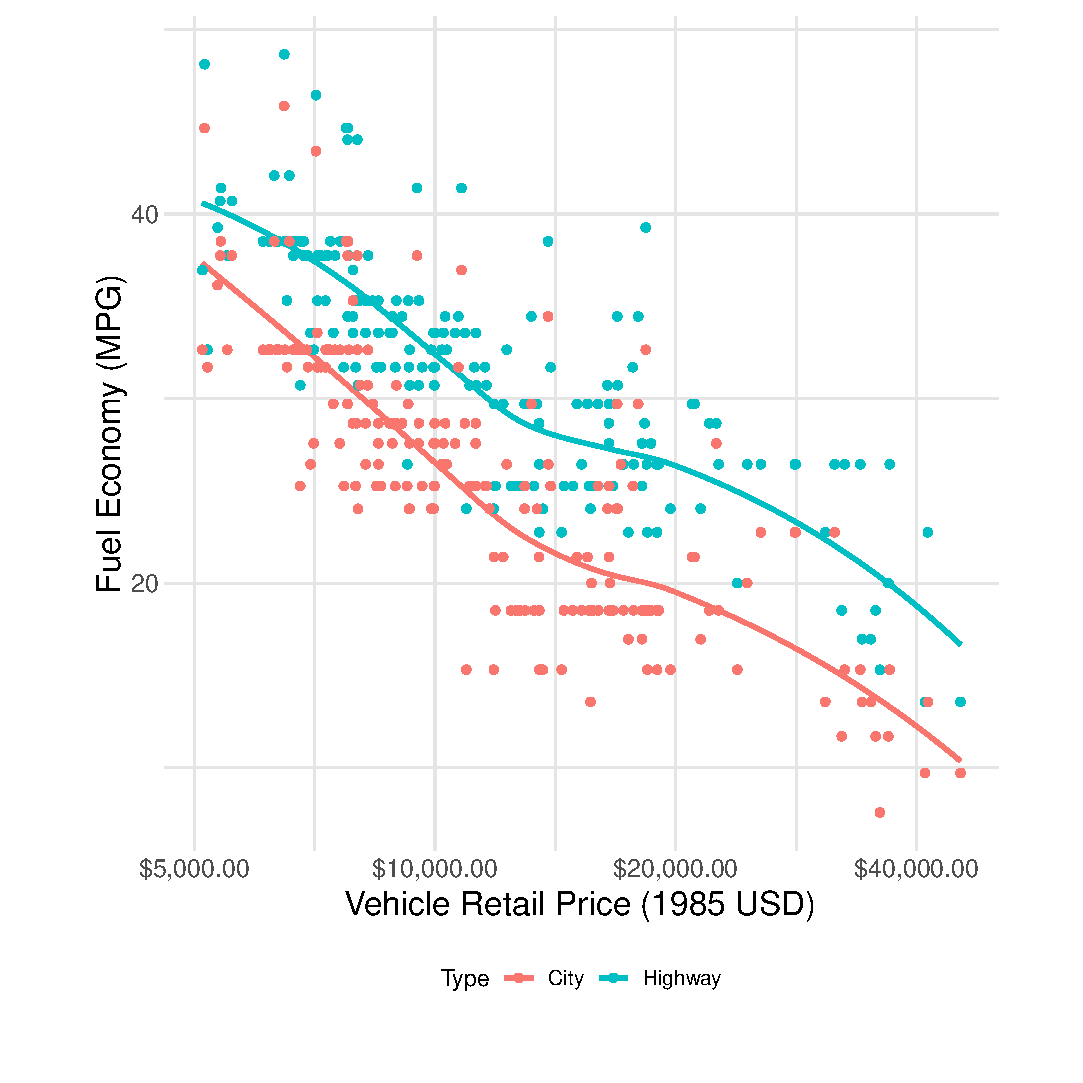
\includegraphics[width=0.90\textwidth]{../images/mpg_vs_usd}
  \caption{Fuel efficiency vs price for the UCI autos dataset.}
  \label{fig:mpg-vs-usd}
\end{figure}

\blfootnote{This -- and all other class materials -- is available at
  https://github.com/zdelrosario/teaching-eda}

\blfootnote{These data are from the UCI Machine Learning database:
  https://archive.ics.uci.edu/ml/index.php}

\end{document}
